% !TEX root = ../my-thesis.tex
%

\chapter{Introducción}
\label{sec:intro}

\cleanchapterquote{El experimentador que no sabe lo que está buscando no comprenderá lo que encuentra.}{Claude Bernard}{(Biólogo teórico, médico y fisiólogo francés.)}


En el presente capítulo se expone el objetivo general, así como sus derivados. En la
primera sección se aborda el tema de investigación donde especifica la justificación del
presente trabajo, posteriormente se sintetiza algunas de las investigaciones que sirvieron
como base para la elección del tema previamente descrito. Finalmente se dan las razones
de la investigación y se exponen las aportaciones derivadas del tema de tesis.

\section{Tema de investigación}
En el campo de la aeronáutica hay una rama que en los últimos años ha sido objeto
de estudio debido a su exponencial importancia para tareas críticas, se trata de los
vehículos aéreos no tripulados UAV (del inglés unmanned aerial vehicle), donde dichas
tareas críticas han podido alcanzar sus objetivos en parte gracias a la implementación
reciente de visión artificial.\\
Sensores como radar, láser y cámaras se han utilizado ampliamente en muchas aplicaciones, como el procesamiento de imágenes, sistemas de rastreo y sistemas de navegación.
En este tipo de sensores, el eje del sensor óptico debe apuntar con precisión desde una base móvil a un objetivo fijo o móvil.\\
En un entorno de este tipo, en el que el equipo suele estar montado en una plataforma móvil, mantener la orientación de los sensores hacia un objetivo es un serio desafío.
Una plataforma de estabilización inercial es una forma apropiada de resolver este desafío.
Este trabajo se centra en el control de una gimbal de dos grados de libertad a través de una cámara montada sobre la plataforma interna de la misma gimbal.

\section{Justificación}
La presente investigación se enfocará en la implementación de una gimbal de dos grados
de libertad utilizando un framework de código abierto y bajo la licencia de Open-Source
siendo este el motivo principal de contribuir a la comunidad y el de la creación de
un repositorio de libre acceso para futuras investigaciones y mejoramiento de la calidad.\\
Para la universidad aeronáutica en Querétaro representará solo el inicio de una potencial
investigación en MAV'S \footnote{Micro air vehicle}.

\section{Objetivo}
%%%%%%%%%%%%%%%%%%%%%%%%%%%%%%%%%%%%%%%%%%%%%%%%%%%%%%%%%%%%%%%%%%%%%%%%%
%Se escribe en infinitivo y resuelve las preguntas ¿Que? ¡Como? y ¿para que? %
%%%%%%%%%%%%%%%%%%%%%%%%%%%%%%%%%%%%%%%%%%%%%%%%%%%%%%%%%%%%%%%%%%%%%%%%%
Diseñar, instrumentar y controlar un dispositivo gimbal que sea capaz de seguir un objeto a través de visión artificial para
implementarse en un UAV de categoría pequeña a velocidad baja.
% \begin{figure}[htb]
% \centering
% 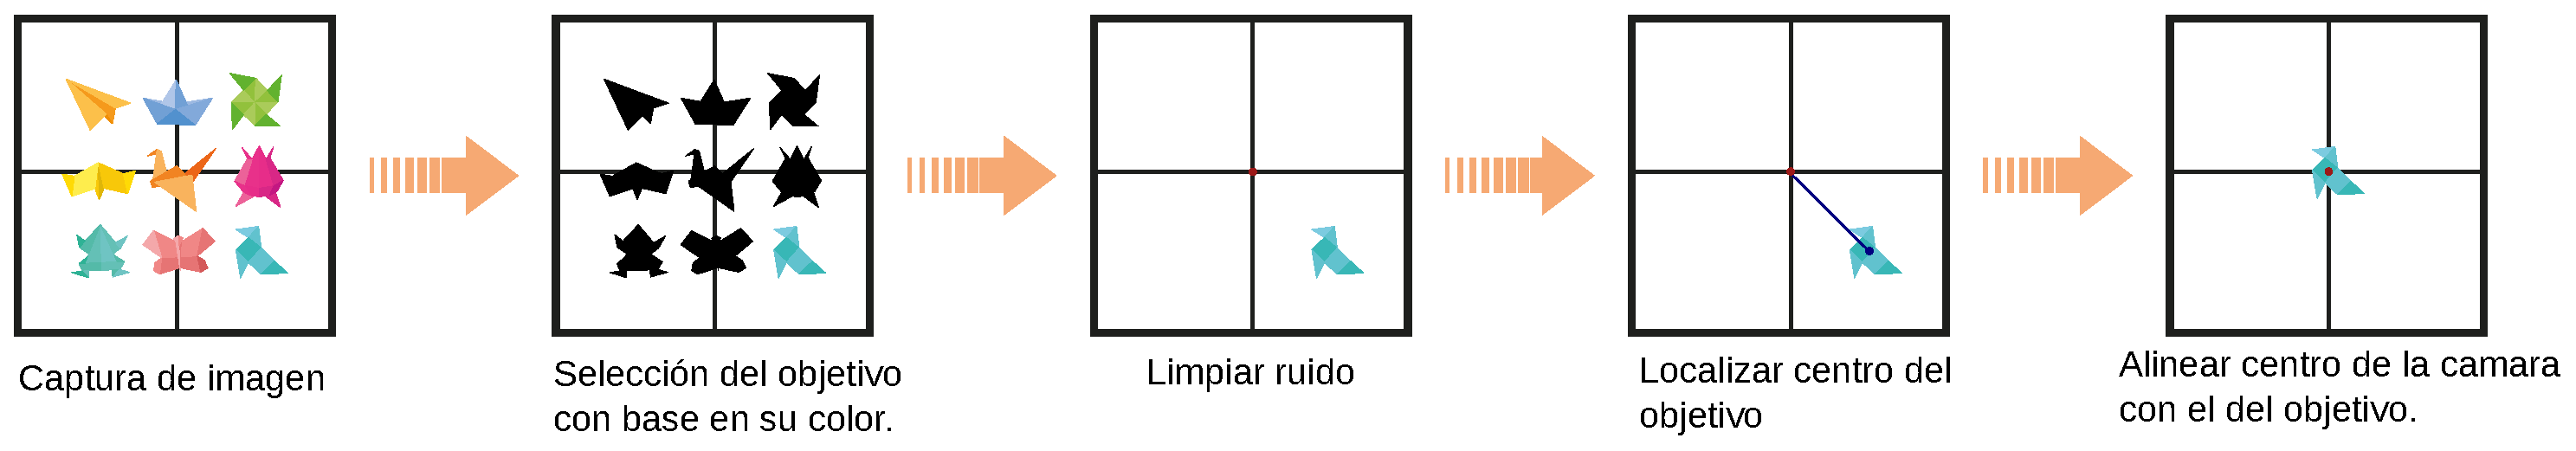
\includegraphics[width=1\textwidth]{Contenido/Cuerpo/Capitulo1/Fig0.eps}
% \captionof{figure}{Representación grafica del objetivo del proyecto}
% \label{fig:Introduccion:Fig1}
% \end{figure}

\section{Objetivos específicos}
%%%%%%%%%%%%%%%%%%%%%%%%%%%%%%%%%%%%%%%%%%%%%%%%%%%%%%%%%%%%%%%%%%%%%%%%%
%Seran los capitulos de la tesis %
%%%%%%%%%%%%%%%%%%%%%%%%%%%%%%%%%%%%%%%%%%%%%%%%%%%%%%%%%%%%%%%%%%%%%%%%%
\begin{itemize}
	\item Definir el modelo matemático de una gimbal con base a los grados de libertad definidos.
	\item Capturar figuras geométricas predefinidas  mediante el uso de una cámara digital y emplear algoritmos de visión artificial para la obtención de datos.
	\item Diseñar e implementar el sistema embebido que dará el soporte electrónico a la gimbal.
	\item Diseñar un controlador autónomo con base en el modelo matemático, previamente obtenido.
\end{itemize}

\section{Estado de la cuestión}
%%%%%%%%%%%%%%%%%%%%%%%%%%%%%%%%%%%%%%%%%%%%%%%%%%%%%%%%%%%%%%%%%%%%%%%%%
%Descripción breve de las obras, proyectos, intentos universitarios más significativos %
%%%%%%%%%%%%%%%%%%%%%%%%%%%%%%%%%%%%%%%%%%%%%%%%%%%%%%%%%%%%%%%%%%%%%%%%%
La aparición de la gimbal no es un término para nada nuevo, de hecho es viejo más de lo que
muchos podemos creer. Fue en el 250 antes de nuestra era cuando el inventor Philo of Byzantium diseño un sistema que pudiera estabilizar la inyección de tinta. \cite{WEB:Gimbal}\\
Desde entonces y hasta la fecha múltiples científicos han desarrollado investigaciones alrededor
de dicho artefacto, algunos teniendo más éxito que otros; los cuales serán brevemente expuestos
con la finalidad de obtener el estado actual en el que se encuentra la gimbal y su avance
tecnológico.
\begin{itemize}
	\item \textbf{Navegación inercial}\\
	      En la navegación inercial, como se aplica a los barcos y submarinos, se necesita
	      un mínimo de tres gimbals para permitir que un sistema de navegación inercial
	      (masa estable) permanezca fijo en el espacio inercial, compensando los cambios
	      en la guiñada, inclinación y balanceo del barco.
	      \begin{figure}[htb]
		      \centering
		      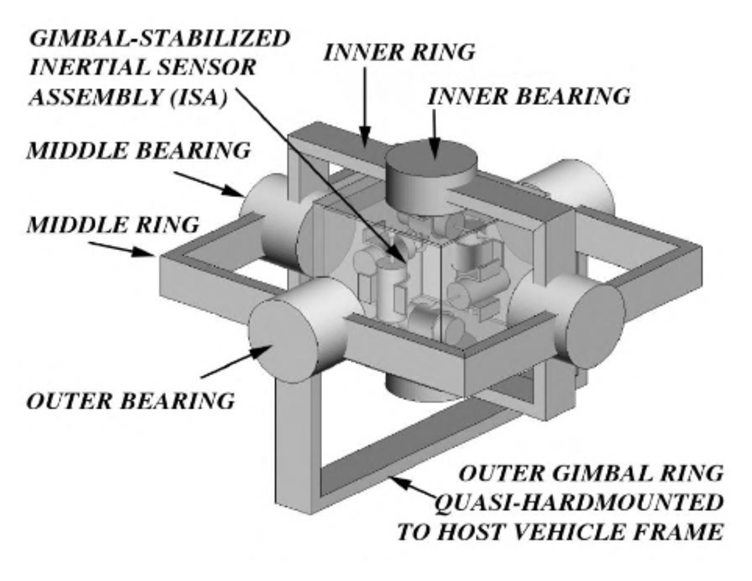
\includegraphics[width=0.6\textwidth]{Contenido/Cuerpo/Capitulo1/Fig1.eps}
		      \captionof{figure}{Uso de una gimbal para un sensor inercial \cite{Book:InNav}}
		      \label{fig:Introduccion:Fig2}
	      \end{figure}

	      En la figura 1.1, la Unidad de medición inercial (IMU) está equipada con tres
	      giroscopios montados ortogonalmente para detectar la rotación alrededor de todos
	      los ejes en el espacio tridimensional. Las salidas giroscópicas accionan motores
	      que controlan la orientación de los tres gimbal según sea necesario para mantener
	      la orientación de la IMU.

	\item \textbf{Motores de cohete}\\
		  En la propulsión de naves espaciales, los motores de cohetes generalmente se
		  montan en un par de gimbals para permitir que un solo motor logre el empuje
		  sobre los ejes de inclinación y guiñada; o, a veces, solo se proporciona un eje
		  por motor. Para controlar el giro, se utilizan motores gemelos con señales de
		  control de inclinación diferencial o guiñada para proporcionar torque sobre el
		  eje de balanceo del vehículo.\\
		  En la figura 1.2 se puede observar uno de los motores más famosos es el J-2X. Es un motor de cohete avanzado altamente
		  eficiente y versátil con las características ideales de empuje y rendimiento para
		  impulsar la etapa superior del espacio de la NASA.\cite{WEB:NASA}
	      \begin{center}
		      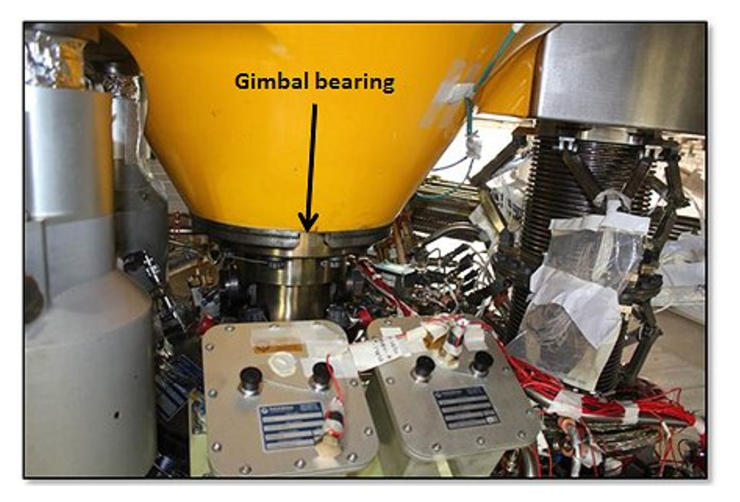
\includegraphics[width=0.65\textwidth]{Contenido/Cuerpo/Capitulo1/Fig2.eps}
		      \captionof{figure}{Uso de una gimbal en un motor de propulsión \cite{WEB:NASA2JX} }
		      \label{fig:Introduccion:Fig3}
	      \end{center}

	\item \textbf{Entrenamiento para astronautas}\\
	      Sistema de simulación de maniobras de tipo caída que se pueden encontrar en el vuelo espacial
	      fue creado por la NASA y era conocido como "the gimbal rig,".
	      Tres jaulas tubulares de aluminio podrían girar por separado o en combinación para
	      dar movimientos de balanceo, cabeceo y guiñada a velocidades de hasta 30
	      revoluciones por minuto, mayores que las esperadas en vuelos espaciales reales.
	      Los chorros de gas nitrógeno, unidos a las tres jaulas, controlaron el movimiento.
	      Desde el 15 de febrero hasta el 4 de marzo de 1960, la plataforma gimbal
	      proporcionó una capacitación valiosa para los siete astronautas del Proyecto
	      Mercurio. Cada uno experimentó unas cinco horas de tiempo de vuelo simulado.\cite{WEB:MERCURY} EN la figura 1.3 se ilustra el sistema antes descrito, que permitió dar un gran
	      paso hacia la capacitación de astronautas.
	      \begin{center}
		      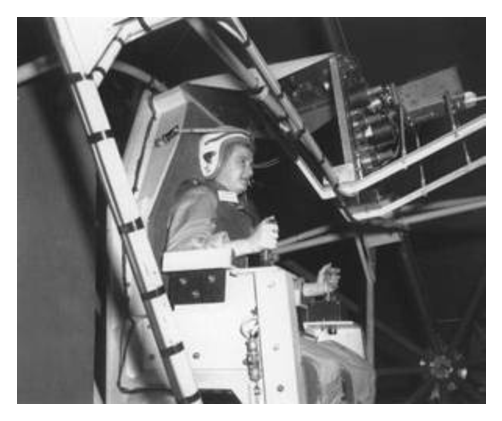
\includegraphics[width=0.45\textwidth]{Contenido/Cuerpo/Capitulo1/Fig3.eps}
		      \captionof{figure}{Jerrie Cobb, uno de los Mercury 13, da un giro en la plataforma gimbal.
			      Créditos: NASA }
		      \label{fig:Introduccion:Fig4}
	      \end{center}

	\item \textbf{Estabilizador de Cámaras}\\
		  Los gimbals también se utilizan para montar todo, desde lentes de cámara pequeñas
		  hasta telescopios fotográficos grandes.\\
		  En los equipos de fotografía portátiles, se utilizan gimbals de un
		  solo eje para permitir un movimiento equilibrado de la cámara y las lentes.
		  Esto resulta útil en la fotografía semi-profesional, así como en cualquier otro
		  caso en el que se adopten teleobjetivos muy largos y pesados: un eje de la gimbal
		  gira un lente alrededor de su centro de gravedad, lo que permite una manipulación
		  fácil y suave mientras se rastrea a los sujetos en movimiento.\\
		  Los montajes de gimbal muy grandes en forma de montajes de altitud-altitud de 2 o 3 ejes
		  se utilizan en la fotografía satelital con fines de seguimiento.\\
		  En la década de 1970, el director de fotografía estadounidense Garrett Brown tuvo
		  una idea simple, pero revolucionaria: hacer un dispositivo que pudiera suavizar las
		  tomas de acción manuales.
	      \begin{center}
		      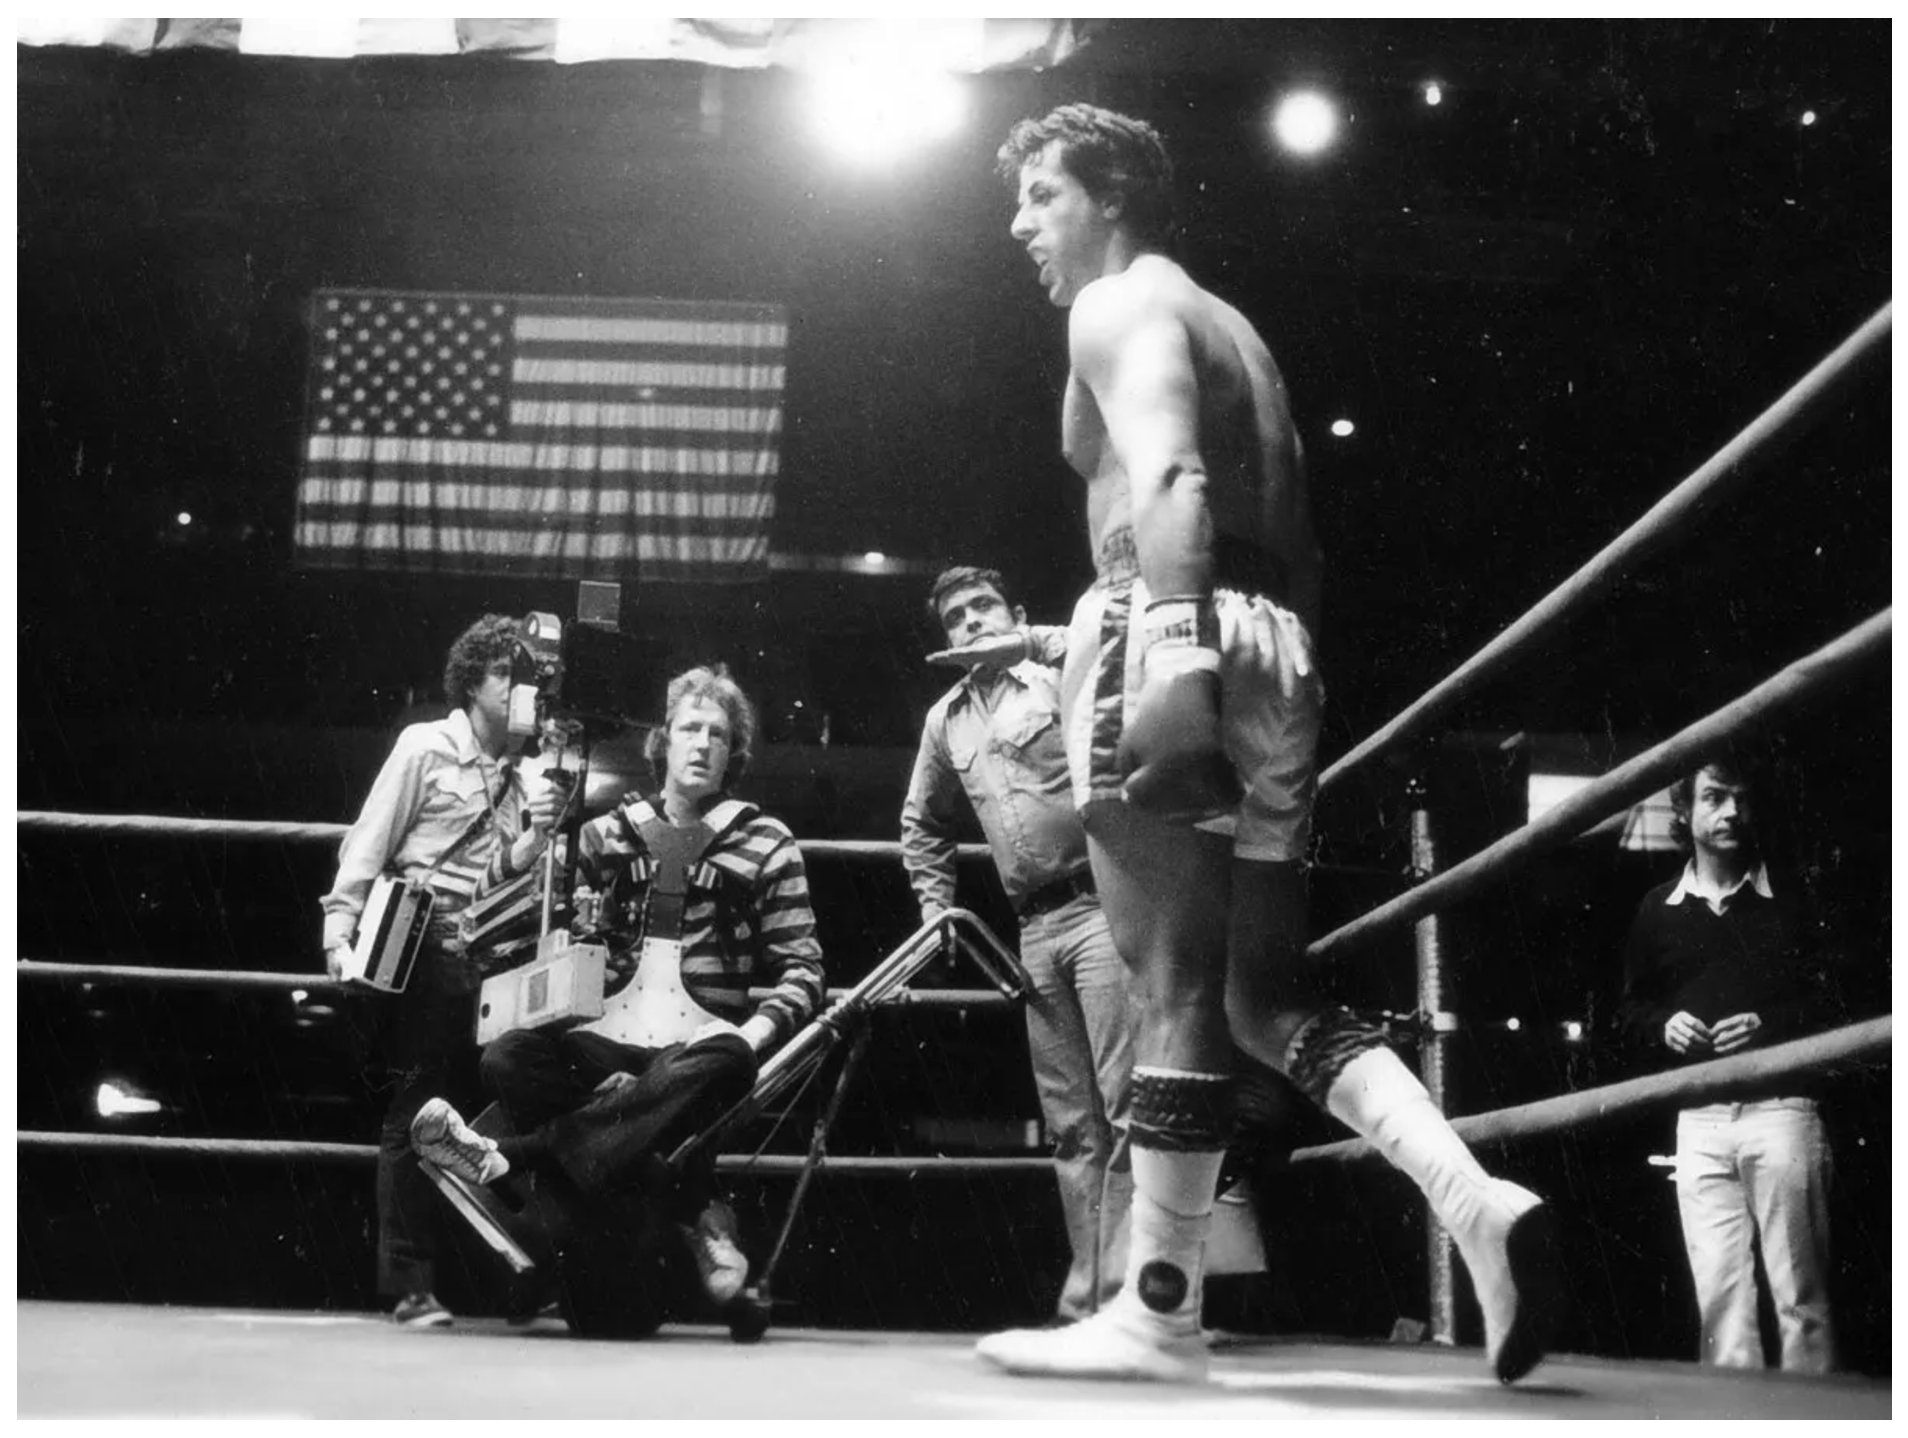
\includegraphics[width=0.45\textwidth]{Contenido/Cuerpo/Capitulo1/Fig4.eps}
		      \captionof{figure}{Primer uso de la steadicam}
		      \label{fig:Introduccion:Fig5}
	      \end{center}

	      El resultado es el Steadicam (Que cumple con los principios físicos de la gimbal).
	      Ganador de un Premio de la Academia, que hizo su debut cinematográfico en la
	      película "Bound for Glory", y se destacó en las películas "Rocky y "The Shining"

	\item \textbf{Control de una gimbal}\\
	      En la literatura se han empleado muchos métodos de control del sistema gimbal de dos ejes. En donde se han propuesto enfoques de agrupación de polos y control óptimo
	      lineal \cite{Paper::Salatun1983},redes neuronales adaptativas de avance multicapa \cite{Paper::Lin2001}, controlador LQG/LTR \cite{Paper::Lee2006} y controlador integral
	      (PI) proporcional\cite{Paper::Kim2010}.

\end{itemize}

\section{Contribuciones}
%%%%%%%%%%%%%%%%%%%%%%%%%%%%%%%%%%%%%%%%%%%%%%%%%%%%%%%%%%%%%%%%%%%%%%%%%
%                         Contribuciones                                %
%%%%%%%%%%%%%%%%%%%%%%%%%%%%%%%%%%%%%%%%%%%%%%%%%%%%%%%%%%%%%%%%%%%%%%%%%
Actualmente la forma en que se desarrollan los sistemas gimbal es mediante el uso de una IMU y cámara, para posteriormente aplicar algún control, en este trabajo se enfoca en omitir
la IMU y hacer la retroalimentación por medio de la cámara, esto nos permite tener un ahorro económico al momento de diseñar el sistema, además de dar otra aproximación al
algoritmo de búsqueda de centroide de la visión artificial, mediante el uso de corrección de factor gamma. Lo que nos puede permitir ajustar los filtros con un sensor de luminancia\\
A nivel escolar, es la primera tesis que incluye visión artificial en la carrera de Ingeniería Electrónica y Control de Sistemas de Aeronaves,
siendo esta investigación el inicio de un proyecto de instrumentación de Vehículos Aéreos no Tripulados con la incorporación de una tarjeta monoprocesador con ROS.

\section{Alcances}
Se tendrá un sistema de control de dos grados de libertad capaz de seguir un objeto de color sólido y geometría conocida en un ambiente controlado, el sistema hará uso
de filtros morfológicos (solo opening y closing) y sé verá limitado por la corrección del brillo mediante software y no hardware.
